\begin{enunciado}{\ejercicio}
    Si hay 3 rutas distintas para ir de Buenos Aires a Rosario, 4 rutas
    distintas para ir de Rosario a Santa Fe, y 2 para ir de Santa Fe a
    Reconquista cuantos formas distintas hay para ir de Buenos Aires a
    Reconquista pasando por las dos ciudades intermedias?
\end{enunciado}

Es un ejercicio bastante directo, queremos ir de Buenos Aires a Reconquista 
pasando por todas las cuidades intermedias, el enunciado no pone ninguna restriccion ni 
atajo de rutas, asi que simplemente multiplicamos todas las posibles rutas. Quedando
$\cajaResultado{3\cdot4\cdot2 = 24}$
\par\bigskip

% es un asco como arme este diagrama jaja pero bueno
\begin{center}
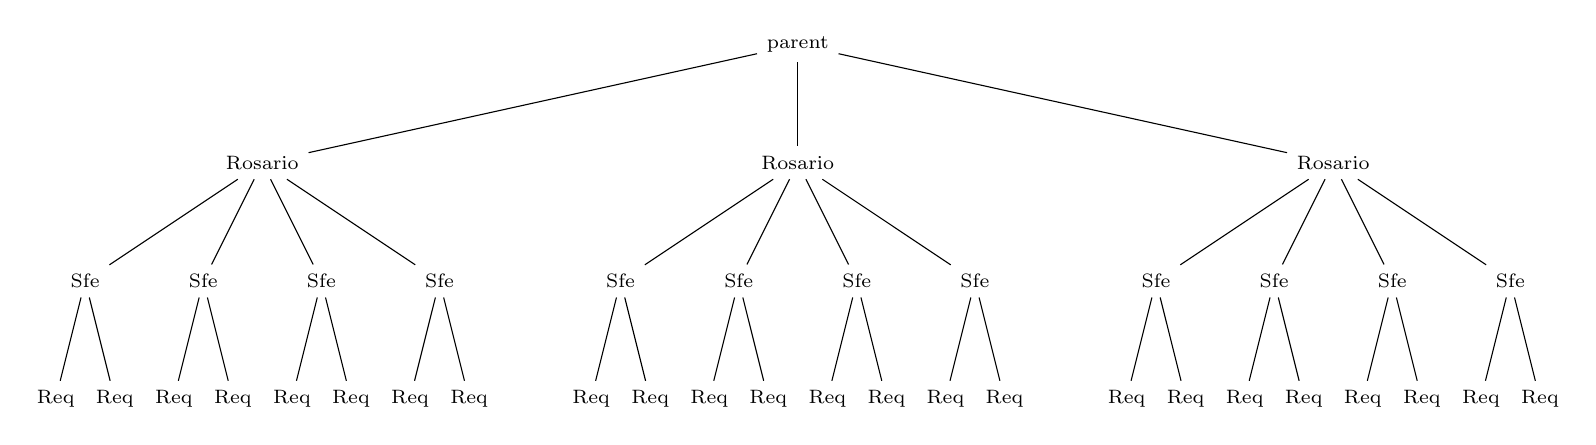
\begin{tikzpicture}[
    level 1/.style = {sibling distance = 6.8cm},
    level 2/.style = {sibling distance = 1.5cm},
    level 3/.style = {sibling distance = 0.75cm},
    every node/.style={font=\scriptsize}
]
    \node {parent}[sibling distance = 5cm]
        child {node {Rosario}
        child {node {Sfe}
        child {node {Req}}
        child {node {Req}}}
        child {node {Sfe}
        child {node {Req}}
        child {node {Req}}}
        child {node {Sfe}
        child {node {Req}}
        child {node {Req}}}
        child {node {Sfe}
        child {node {Req}}
        child {node {Req}}}}
        child {node {Rosario}
        child {node {Sfe}
        child {node {Req}}
        child {node {Req}}}
        child {node {Sfe}
        child {node {Req}}
        child {node {Req}}}
        child {node {Sfe}
        child {node {Req}}
        child {node {Req}}}
        child {node {Sfe}
        child {node {Req}}
        child {node {Req}}}}
        child {node {Rosario}
        child {node {Sfe}
        child {node {Req}}
        child {node {Req}}}
        child {node {Sfe}
        child {node {Req}}
        child {node {Req}}}
        child {node {Sfe}
        child {node {Req}}
        child {node {Req}}}
        child {node {Sfe}
        child {node {Req}}
        child {node {Req}}}};
    

\end{tikzpicture}
\end{center}

Como se ve en ese diagrama de decision, hay $\cajaResultado{24}$ formas de llegar a reconqusita desde Buenos Aires.

\begin{aportes}
    \item \aporte{https://github.com/sigfripro}{sigfripro \github}
\end{aportes}